\documentclass[12pt]{article}
\usepackage[utf8]{inputenc}
\usepackage[T1]{fontenc}
\usepackage{amsmath,amssymb}
\usepackage{mathptmx}
\usepackage{booktabs}
\usepackage{url}
\urlstyle{same}
\usepackage{graphicx}
\usepackage[margin=1in]{geometry}
\usepackage{setspace}
\usepackage{titlesec}
\usepackage{indentfirst}
\usepackage{float}
\usepackage{caption}
\usepackage{ragged2e}
\captionsetup{
  labelsep = newline,
  labelfont = bf,
  textfont = it,
  justification = raggedright,
  singlelinecheck = false
}
\captionsetup[figure]{textfont={}}

\newcommand{\code}[1]{\textit{#1}}
\newcommand{\soft}[1]{\textnormal{#1}}

% APA 7 formatting
\doublespacing
\RaggedRight
\setlength{\parindent}{0.5in}
\setlength{\parskip}{0pt}

% APA headings: Level 1 (centered, bold) and Level 2 (flush left, bold), unnumbered
\titleformat{\section}{\centering\normalfont\normalsize\bfseries}{}{0em}{}
\titleformat{\subsection}{\normalfont\normalsize\bfseries}{}{0em}{}
\titlespacing*{\section}{0pt}{0pt}{0pt}
\titlespacing*{\subsection}{0pt}{0pt}{0pt}

\begin{document}

\pagenumbering{gobble}

\begin{center}
  \vspace*{1in}

  \textbf{Predicting Loneliness Beyond Social Contact Frequency: Evidence from ESS Round 7}

  \vspace{\baselineskip}

  Shuxuan Chi and Hongyi Huang

  Department of Psychology, Chinese University of Hong Kong

  PSYC6000: Psychological Approaches

  Dr. Xianming GONG

  November 1, 2026
\end{center}

\vfill

\begin{center}
  \textbf{Author Note}
\end{center}

LLMs such as ChatGPT were used to assist with clarifying machine-learning questions, reviewing R code, 
improving the clarity and readability of the manuscript, and providing critical feedback on the analytical 
approach. The authors evaluated the suggestions and all final decisions regarding the analyses, reporting, 
and wording choices were made by the authors, who take full responsibility for the content of this manuscript.

This manuscript contains 3,835 words in total. The word count by section is: 
Introduction, 726; Methods, 900; Results, 741; Discussion, 943; Conclusion, 126; and References, 399.
% Abstract, 176; 

Analysis scripts, the data, and the original figures
presented in this manuscript are available at github repository: \url{https://github.com/DerrickHHY/PSYC_6000_Social}.
\newpage

\section{Abstract}

Loneliness can occur despite frequent social contact, but it remains unclear whether other
social indicators improve prediction beyond contact frequency. Using European Social
Survey Round 7 data ($N = 37{,}868$; 21 countries), we examined whether confidant
availability and perceived social activity relative to age peers improve prediction of
concurrent loneliness for new respondents. Incremental analyses used nested ordinal
forests in a subsample of 10,500 respondents, testing each indicator separately and
jointly against a baseline comprising meeting frequency and background characteristics.
Adding both indicators to meeting frequency and background characteristics increased
quadratic-weighted $\kappa$ from $.182$ to $.204$, whereas separate additions yielded
small, inconsistent changes. Accuracy and mean absolute error changed little. Exploratory
analysis of the full-sample forest identified household size, age, income strain, and
self-rated health as prominent predictors. These findings indicate a modest joint
contribution from relational resources and comparative social evaluations. Direct
assessment of unmet relational needs may help clarify whether more differentiated social
measurement improves loneliness prediction and informs research on support matched to
those needs.

\textit{Keywords:} loneliness, social connection, confidant availability, social
comparison, incremental prediction, ordinal forest

\newpage

\pagenumbering{arabic}

\section{Introduction}

Addressing loneliness is important for human well-being, but understanding it requires
looking beyond whether people are alone. People may feel connected while alone, or lonely
despite regularly meeting friends, relatives, or colleagues. Beyond contact frequency, the
opportunities for personal connection within these relationships and people's own
evaluations of their social lives may help us understand why. This emphasis on subjective
experience is central to the distinction between loneliness and objective social isolation
(Hawkley \& Cacioppo, 2010). Perlman and Peplau's (1981) discrepancy account proposed that
loneliness arises when people's relationships fall short of what they desire, whether in
quantity or quality. From this perspective, people may experience similar levels of
contact differently, depending on the connections available to them and the standards they
use to evaluate them.

Contact frequency remains a useful starting point. Luhmann and Hawkley (2016) found that
quantitative indicators of social relationships, including contact frequency, were
associated with loneliness across age groups in a large German sample. Other research
suggests that people's evaluations of their contact also deserve attention. Examining
friendship among Norwegian adults aged 18--79, Nicolaisen and Thorsen (2017) considered
actual contact alongside confidant friendships, satisfaction with contact, and aspirations
for contact. Dissatisfaction with contact was strongly associated with loneliness across
the age groups examined. Given the broad age range examined in the present study, we
consider age and relevant life circumstances when assessing what relational resources and
comparative evaluations contribute beyond contact frequency.

The standards underlying the evaluations have also been examined directly. Across two
cross-sectional studies in five European countries, Heu et al.\ (2019) investigated
discrepancies between actual relationships and personal or socially perceived
expectations. Their second study assessed contact frequency and relationship quality
involving partners, close family members, and best friends, together with corresponding
desired and normative relationship characteristics. Larger discrepancies between ideal
and actual relationships were associated with greater loneliness.

The European Social Survey (ESS), a cross-national survey of social attitudes, beliefs,
and behavior, brings these questions into focus through measures of meeting frequency,
confidant availability, and perceived social activity relative to peers of the same age.
The last of these introduces a specific comparative perspective: respondents assess how
socially active they are compared with others of the same age. This differs from the
desired--actual discrepancies examined by Heu et al.\ (2019), but similarly directs
attention to how people evaluate their social circumstances alongside their reported
contact.

Using ESS Rounds 3, 5, 6, and 7 from 17 countries, Amendola and von Wyl (2025) examined
these three indicators together. They measured confidence-based emotional support by
whether respondents had at least one person they could discuss intimate and personal
matters with. After adjusting for sociodemographic characteristics, emotional support,
meeting frequency, and peer-relative social activity were each associated with lower
loneliness, although the meeting and activity associations were very small or negligible.

These findings establish associations, but leave a more specific predictive question
unanswered: once meeting frequency and background characteristics are known, do confidant
availability and peer-relative social activity improve predictions of loneliness for new
respondents? An indicator can be associated with loneliness yet contribute little
additional predictive information if its information overlaps with what other
characteristics already provide. Yarkoni and Westfall (2017) emphasized evaluating
psychological models on new observations and discussed comparisons between predictor sets
as a way to examine their contributions. The distinction between association and
predictive usefulness is therefore central to the present study.

Using ESS Round 7, the present study asks whether knowing how many people someone can
confide in, and how socially active they consider themselves relative to age peers,
improves prediction of loneliness beyond knowing how often they meet others and their
background characteristics. We expect both indicators to provide additional predictive
information. We evaluate their contributions separately and jointly against a baseline
that includes meeting frequency, household size, age, gender, education, income strain,
and self-rated health. A complementary interpretation of the full-sample model examines
predictor importance and prediction profiles within respondents' wider life
circumstances.

The study focuses on predicting concurrent loneliness among new respondents from the
countries represented in the sample. The findings may inform how social connection is
assessed in loneliness research by clarifying the added predictive value of confidant
availability and peer-relative social activity beyond contact frequency. In the longer
term, this evidence could help formulate hypotheses for intervention research on access
to confidants and social participation alongside opportunities for contact.

\section{Methods}

\subsection{Data and participants}

Data come from the European Social Survey Round~7 (ESS7), integrated file, edition~2.3
(ESS ERIC, 2014). The integrated file contains $N=40{,}185$ respondents nested within
$21$ countries. After the data preparation, $N=37{,}868$ respondents remained for analysis.

\subsection{Measures}

\textit{Outcome.} Loneliness was measured with a single item asking how often the respondent
\textit{felt lonely during the past week} (\code{fltlnl}), answered on a four-point ordinal
scale ($1 =$ none or almost none of the time, $2 =$ some of the time, $3 =$ most of the
time, $4 =$ all or almost all of the time). Higher values indicate more frequent loneliness.

\textit{Predictors.} Two social-connection predictors captured the focal indicators whose
incremental predictive contribution was of primary interest: \code{inprdsc} (number of people
with whom the respondent can discuss intimate and personal matters; $0$--$6$) and \code{sclact}
(how often the respondent takes part in social activities compared with others of the same age;
$1$--$5$). All remaining predictors served as covariates, against which the incremental
contribution of the two social-connection predictors was assessed: social meeting frequency
(\code{sclmeet}; how often the respondent meets socially with friends, relatives, or
colleagues; $1$--$7$), household size (\code{hhmmb}; the number of people, where a value of $1$ indicates living alone),
age in years (\code{agea}), gender (\code{gndr}; male/female), years of full-time education
completed (\code{eduyrs}), feeling about the household's current income (\code{hincfel};
$1$--$4$, from living comfortably to very difficult), and self-rated health (\code{health};
$1$--$5$, from very good to very bad). The respondent's country of residence (\code{cntry})
served as the grouping variable for the random intercept. Table~\ref{tab:measures} summarizes
the measures.

\begin{table}[H]
\footnotesize
\caption{Measures Used in the Analysis}
\label{tab:measures}
\begin{tabular}{llll}
\toprule
ESS code & Measure & Scale / levels & Role \\
\midrule
\code{fltlnl} & Felt lonely, past week & 1--4 & Outcome (ordinal) \\
\code{inprdsc} & Confidants (intimate discussion) & 0--6 & Social-connection predictor \\
\code{sclact} & Social activity vs.\ age peers & 1--5 & Social-connection predictor \\
\code{sclmeet} & Social meeting frequency & 1--7 & Covariate \\
\code{hhmmb} & Household size & count & Covariate \\
\code{agea} & Age (calculated) & years & Covariate \\
\code{gndr} & Gender & male/female & Covariate \\
\code{eduyrs} & Years of full-time education & years & Covariate \\
\code{hincfel} & Feeling about household income & 1--4 & Covariate \\
\code{health} & Subjective general health & 1--5 & Covariate \\
\code{cntry} & Country of residence & 21 countries & Grouping (random intercept) \\
\bottomrule
\end{tabular}

\vspace{6pt}

\raggedright
\textit{Note.} ESS = European Social Survey.
\end{table}

\subsection{Data preparation}

Following the ESS codebook, missing-value codes were recoded to NA ($77/88/99$: 
\code{sclmeet}, \code{inprdsc}, \code{eduyrs}, \code{hhmmb}; $7/8/9$: \code{fltlnl}, \code{sclact}, 
\code{hincfel}, \code{health};$9$: \code{gndr}; $999$: \code{agea}). Gender and country were converted 
to factors, and the outcome \code{fltlnl} was treated as an ordered factor.
Observations with any missing value on the analysis variables were removed by listwise
deletion, leaving $N=37{,}868$ observations. 


\subsection{Prediction models}

This project fitted four computational models in a fully crossed $2 \times 2$ design, 
crossing individual-level functional form (linear vs. nonlinear) with 
the treatment of country clustering (a random intercept vs. no random effects): a) the cumulative link 
model (CLM; McCullagh, 1980), a proportional-odds
model with linear fixed effects and no random effects; b) the cumulative link mixed
model (CLMM; Tutz \& Hennevogl, 1996), the CLM extended with a country-level random intercept; c) the
ordinal forest (OF; Hornung, 2020), a tree-based ensemble for ordinal responses that captures
nonlinear fixed effects and no random effects; and d) ordinal
mixed-effects random forests (OMERF; Bergonzoli et al., 2026), a tree-based model that estimates the fixed component
with a random forest while capturing a random intercept. 
A majority-class baseline, which predicts the most frequent training-set category
for every observation, was included as a no-information reference.

All models shared the same inputs and output: nine predictors (\code{sclmeet},
\code{inprdsc}, \code{sclact}, \code{hhmmb}, \code{agea}, \code{gndr}, \code{eduyrs},
\code{hincfel}, and \code{health}) and the four-category loneliness outcome
(\code{fltlnl}); the mixed models additionally included country (\code{cntry}) as a random
intercept.

All models were estimated in \soft{R} (R Core Team, 2025). OMERF was fitted with the reference implementation of
Bergonzoli et al.\ (2026), which is initialized by an ordinal forest and then iteratively
alternates between a random forest for the fixed component (via the \soft{ranger} package,
Wright \& Ziegler, 2017) and a cumulative link mixed framework for the random intercept (via the
\soft{ordinal} package, Christensen, 2022); convergence required the maximum relative change in 
estimated random effects between consecutive iterations to fall below $.1$, more lenient than the default of $.05$.
CLM and CLMM were fitted with the \soft{clm} and \soft{clmm} functions of the
\soft{ordinal} package using the logit link. The ordinal forest was fitted with the \soft{ordfor} function of the
\soft{ordinalForest} package (Hornung, 2020), with default hyperparameters (e.g., $500$ trees).

\subsection{Model evaluation and selection}

Predictive performance was assessed with five-fold cross-validation. Country was used as the stratification 
variable so that each fold reflected the country composition of the full analytic sample. Each model was 
trained on four folds and evaluated on the held-out fold, and performance was averaged across the five folds.

Model performance was summarized with three complementary measures: accuracy, the
quadratic-weighted Cohen's $\kappa$ (Cohen, 1968), and mean absolute error (MAE). Accuracy
is the proportion of exactly correct predictions but treats every error as equally severe and
can be uninformative when the response is skewed. The $\kappa$ penalizes disagreements
by the squared distance between the category ordinal values, so that misclassifications
between more distant categories are weighted more heavily. MAE, computed on the integer category
labels, is the average number of categories by which a prediction deviates from the observed
response (lower is better). 
% Together, MAE and weighted $\kappa$ capture error magnitude and ordinal agreement beyond what accuracy alone reveals.

To quantify between-country heterogeneity, the intraclass correlation coefficient (ICC) of
the mixed models was computed from a full-sample fit as
$\mathrm{ICC} = \sigma^{2} / \left(\sigma^{2} + \pi^{2}/3\right)$ (Grilli \& Rampichini,
2011). Model selection combined the ICC magnitude with
the cross-validated predictive performance: an ICC below $.05$ would indicate
negligible country-level clustering and favor the fixed-effects models.

On the basis of these metrics, a single model structure was selected for subsequent analysis. 
The selected model was fitted to the full sample, and its outputs were used for interpretation 
(variable importance: random 1,000-respondent subsample; partial dependence: full sample).

\subsection{Incremental predictive value}

To assess the incremental predictive value, we compared four nested models (identical structure, varying predictors)
refitted on a random subsample of 500 respondents per country (N = 10,500). M1 served as the baseline (background covariates only);
M2 added \code{inprdsc}, M3 added \code{sclact}, and M4 added both. Using the same five-fold partition, we computed accuracy, 
$\kappa$, and MAE per fold and compared ($M_2$--$M_4$) against M1.

\section{Results}

\subsection{Outcome distribution}

Figure~\ref{fig:outcome} shows the distribution of the loneliness outcome. The outcome
was strongly skewed: $70.8\%$ of respondents reported feeling lonely none or almost none
of the time, $22.3\%$ some of the time, $4.7\%$ most of the time, and $2.3\%$ all or
almost all of the time.

\begin{figure}[H]
  \caption{Distribution of the Four-Category Loneliness Outcome}
  \label{fig:outcome}
  \centering
  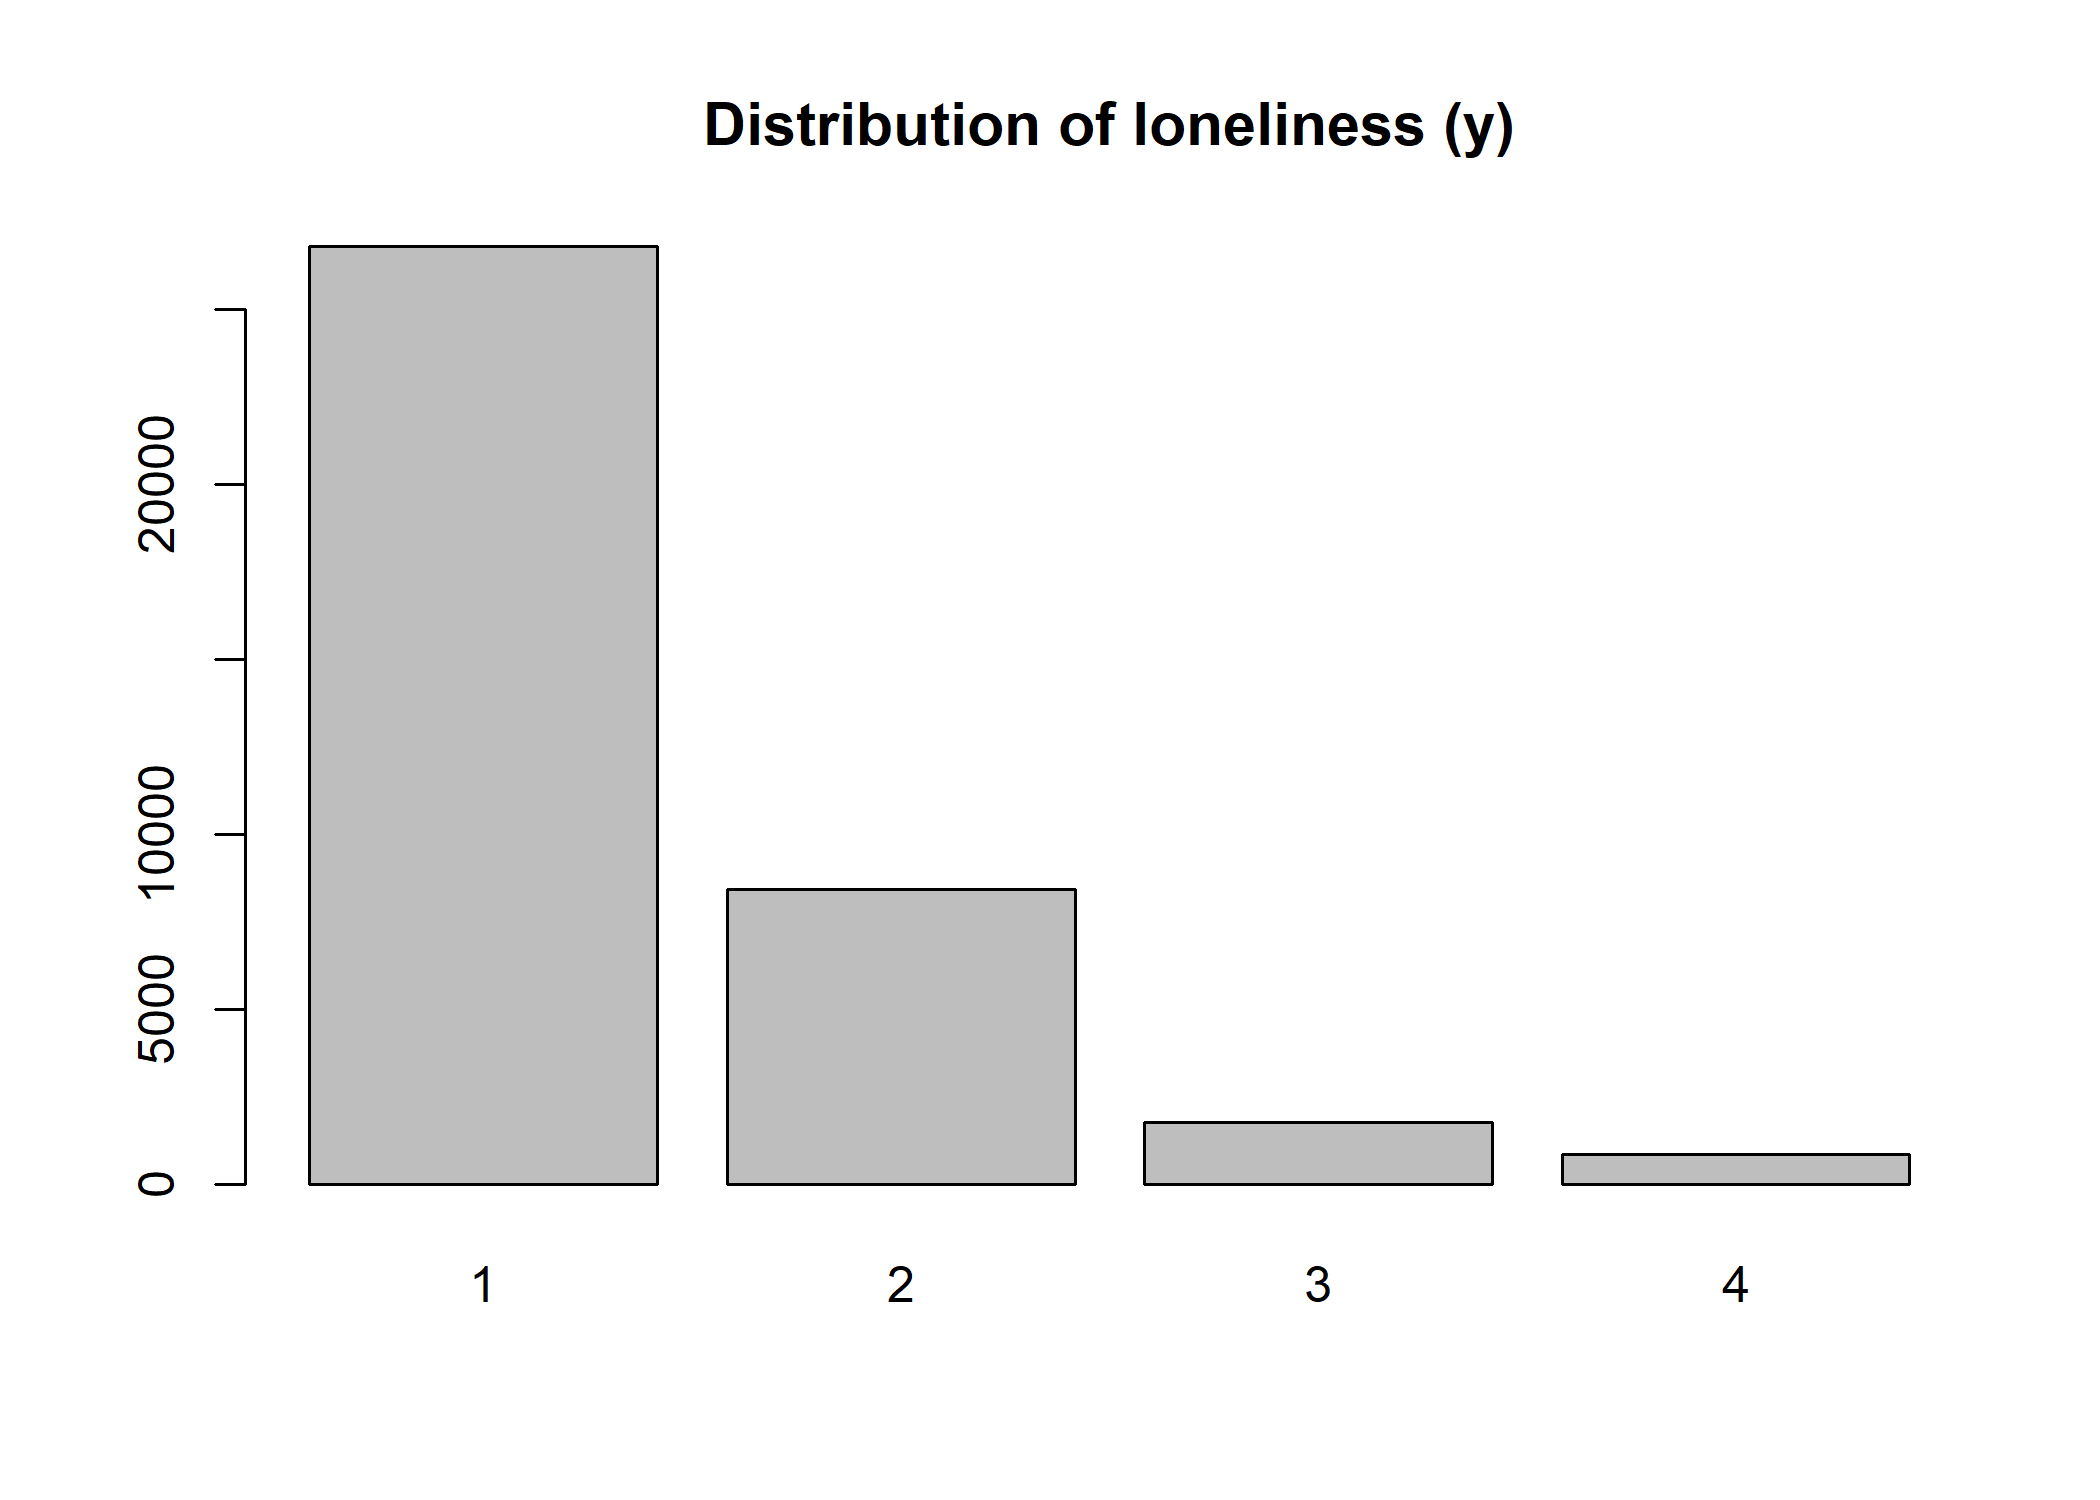
\includegraphics[width=0.65\textwidth]{fig_y_dist.png}

  \raggedright
  \textit{Note.} The x-axis reports the four loneliness categories (1 = none or almost 
  none of the time; 2 = some of the time; 3 = most of the time; 4 = all or almost all 
  of the time).
\end{figure}

\subsection{Predictive performance and model selection}
Given the pronounced skewness, a majority-class baseline model achieves an accuracy of $.708$ by merely predicting option 1. 
Against this reference, the four models achieved only comparable accuracy ($.707$--$.714$; Table~\ref{tab:comparison}).
Accuracy is therefore uninformative here, because of the pronounced skewness.
% notably, OMERF's accuracy ($.707$) fell slightly below the majority-class baseline.


\begin{table}[H]
  \footnotesize
  \caption{Predictive Performance of the Compared Models}
  \label{tab:comparison}
  \begin{tabular}{lcccccc}
    \toprule
    Model & Accuracy & Weighted $\kappa$ & MAE & ICC & Trees & Convergence \\
    \midrule
    Majority (baseline) & .708 (.002) & .000 & .384 (.004) & -- & -- & -- \\
    OMERF & .707 (.003) & .059 (.013) & .380 (.005) & .047 & 5000 & Conv.\ (5 it.) \\
    CLMM  & .714 (.003) & .171 (.014) & \textbf{.355} (.004) & .0227 & -- & No warnings \\
    CLM   & .712 (.003) & .155 (.008) & .359 (.005) & -- & -- & No warnings \\
    Ordinal forest & .714 (.004) & \textbf{.214} (.019) & .356 (.005) & -- & 500 & No warnings \\
    \bottomrule
  \end{tabular}

  \vspace{6pt}

  \raggedright
  \textit{Note.} Accuracy, quadratic-weighted Cohen's $\kappa$, and MAE are means across five test
  folds (standard deviations in parentheses). MAE = mean absolute error; ICC = intraclass
  correlation coefficient. CLM and CLMM are linear models with no tree hyperparameters.
\end{table}

The ordinal forest achieved the highest $\kappa$ ($.214$), followed by the CLMM ($.171$) and the CLM
($.155$), whereas OMERF's $\kappa$ ($.059$) was markedly lower. Although CLMM attained the lowest MAE
 ($.355$) and the highest accuracy ($.714$), the ordinal forest was nearly identical (MAE $.356$). 
 The country random intercept explained little variance (ICC $= .047$ for OMERF and $.023$ for CLMM), indicating weak
country-level clustering. Consequently, the ordinal forest was selected as the reference model due to its superior 
 $\kappa$ and accuracy and MAE comparable to those of CLMM.

\subsection{Variable importance}

To examine the underlying predictive patterns, the results in this subsection are derived 
from the ordinal forest fitted on the full sample, with permutation importance computed from 
a random subsample of 1,000 respondents. 

The ranking of variables clearly highlights the dominant role of structural and 
socio-demographic factors over social-behavioral frequency (see Figure~\ref{fig:importance}). Household size (\code{hhmmb}) 
emerged as the most important predictor by a substantial margin, followed by age (\code{agea}), 
feeling about household income (\code{hincfel}), self-rated health (\code{health}), and 
the number of confidants (\code{inprdsc}), which formed a tightly clustered second tier 
of highly important features. These were followed by social activity relative to age peers (\code{sclact}), years 
of education (\code{eduyrs}) and social meeting frequency (\code{sclmeet}). Notably, gender (\code{gndr}) ranked as the least important 
predictor. 

\begin{figure}[H]
  \caption{Permutation Importance of the Predictors in the Ordinal Forest}
  \label{fig:importance}
  \centering
  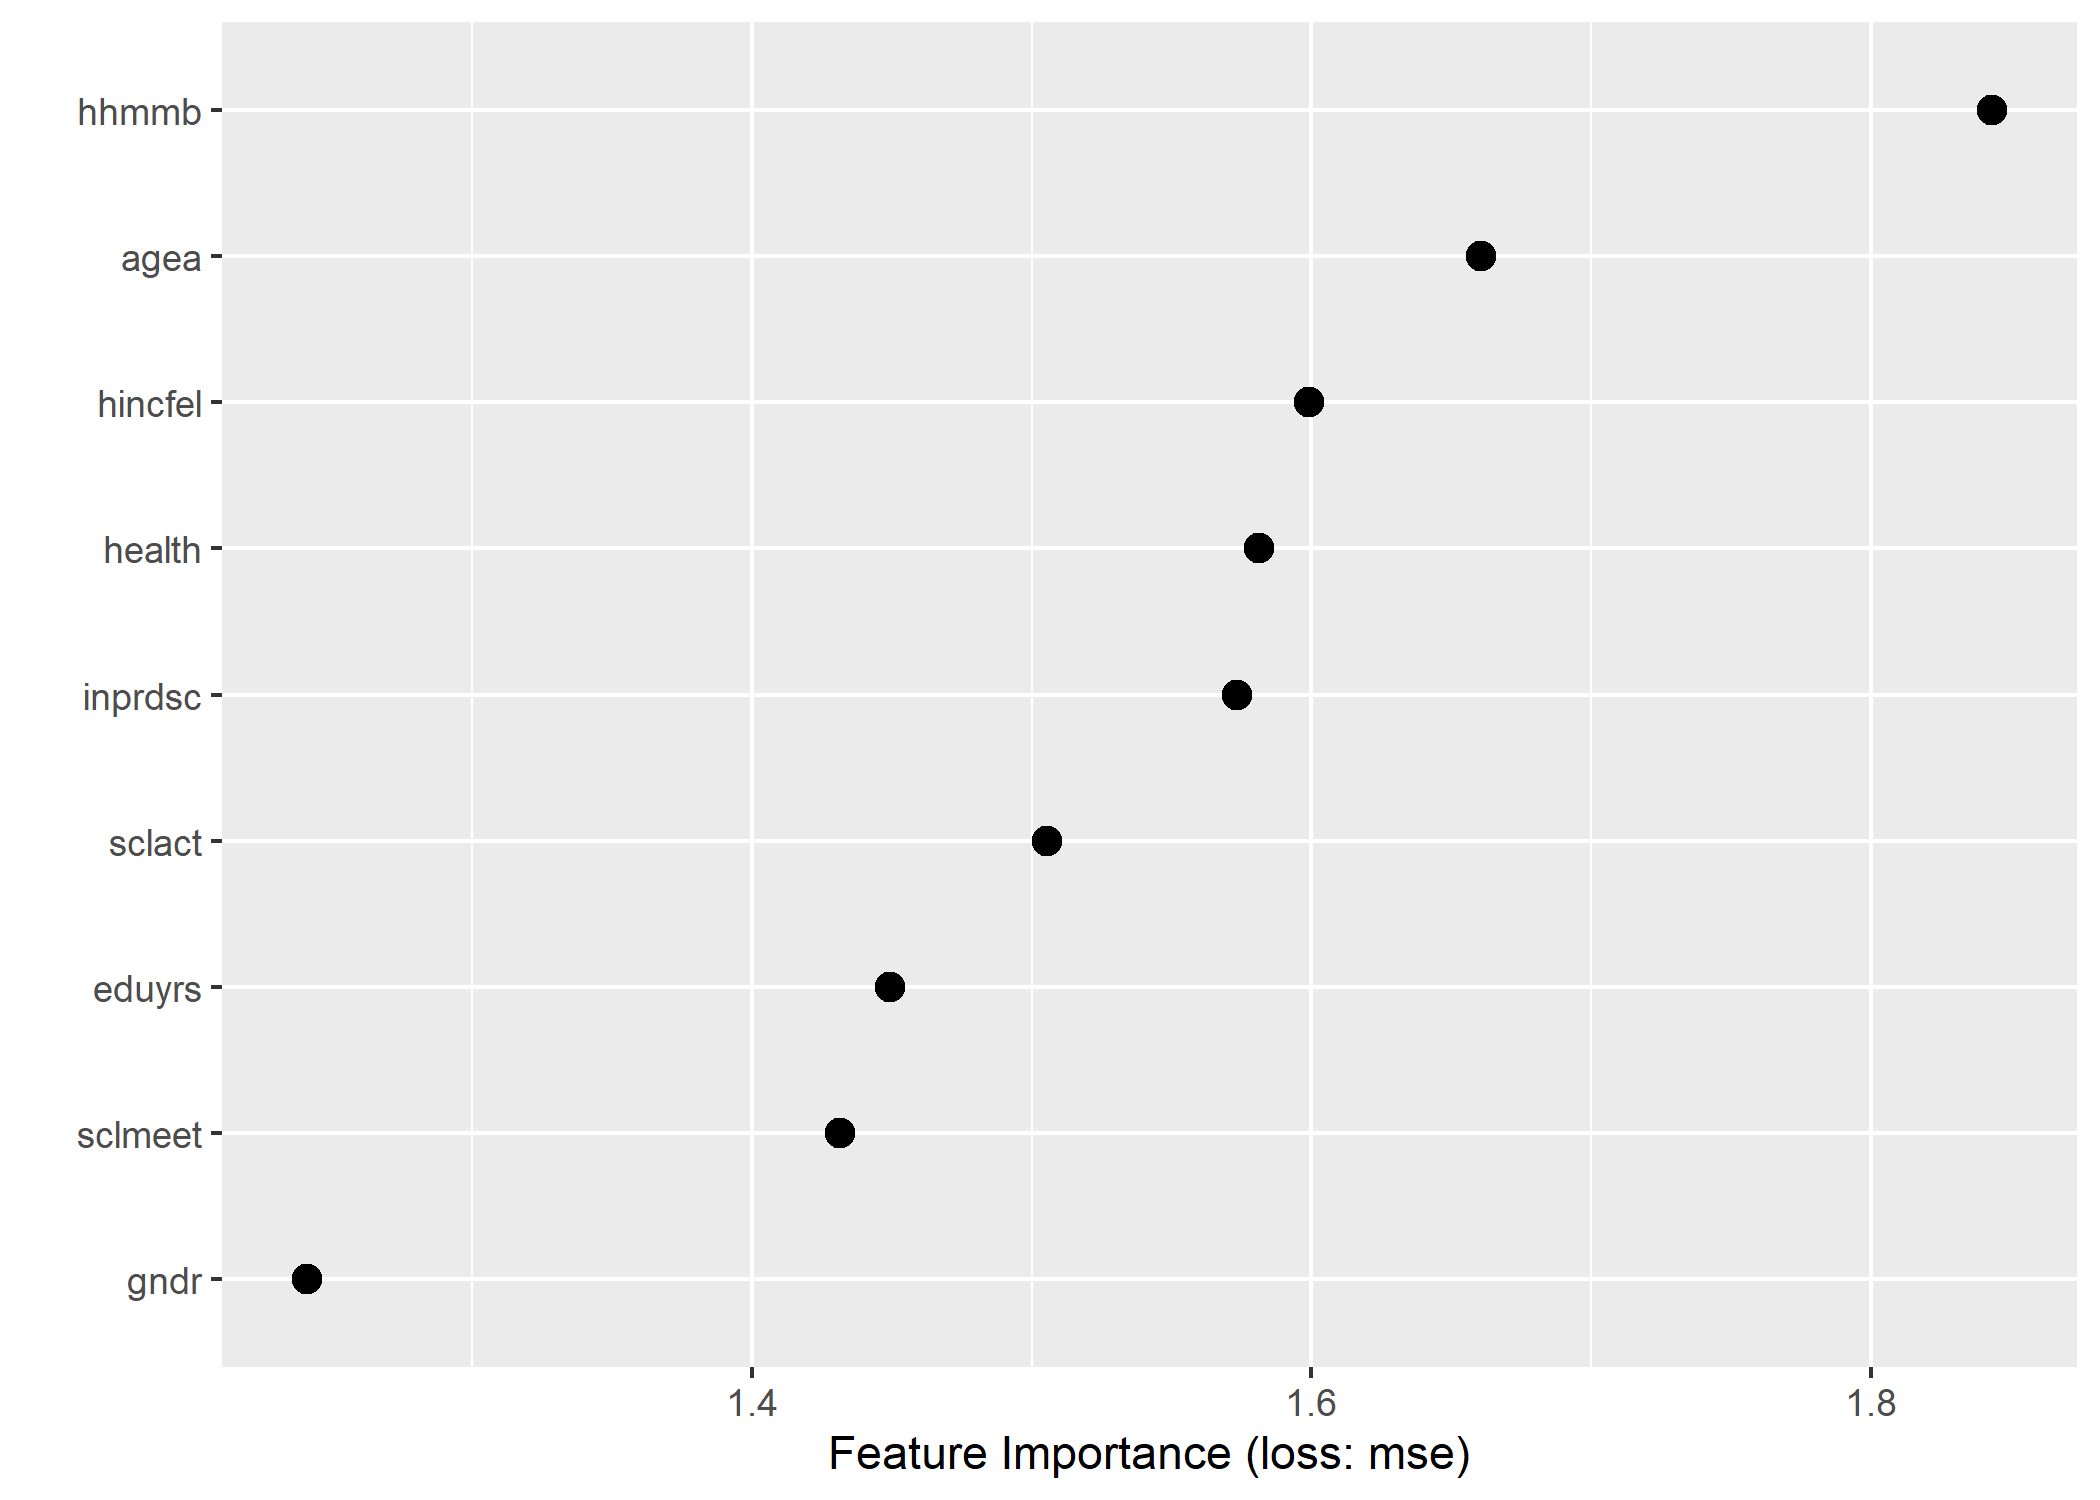
\includegraphics[width=0.8\textwidth]{imp_2_of_full.png}

  \raggedright
  \textit{Note.} The x-axis reports the factor increase in prediction error when each
  predictor is permuted; the y-axis lists the predictors. Computed on a random subsample of
  1,000 respondents.
\end{figure}

\subsection{Partial dependence}

Figure~\ref{fig:pdp} shows partial dependence of expected loneliness for each predictor, 
with the remaining numerical predictors held at their medians and gender held fixed. Higher values 
on the vertical axis indicate more frequent predicted loneliness. For social meeting frequency
(\code{sclmeet}), the association was non-linear: expected loneliness was highest among 
those who never met socially and declined markedly as frequency increased from 
never to moderate levels, after which the curve largely leveled off for higher frequencies. 
Expected loneliness declined with the number of confidants (\code{inprdsc}), with the steepest drop occurring up to two confidants; 
however, the curve showed a slight uptick at the highest categories. 
Similarly, social activity relative to age peers (\code{sclact}) exhibited a decline in 
expected loneliness up to the level of parity with peers. The sharpest reduction occurred 
between categories 1 and 2, after which expected loneliness largely plateaued, showing negligible 
further benefit for those who are more socially active than their peers. For household size (\code{hhmmb}), 
expected loneliness dropped precipitously from one member to three members and then remained remarkably flat for larger households, 
indicating that living with at least one other person acts as a primary buffer against loneliness.

The age trajectory (\code{agea}) displayed a clear U-shaped relationship: expected loneliness 
was relatively high in young adulthood (under 30), reached its lowest and most stable point 
between ages 30 and 60, and then increased steeply after age 60, peaking in the oldest age 
groups (80+). The trajectory for years of education (\code{eduyrs}) was non-linear: 
expected loneliness dipped initially (from 0 to roughly 10 years), rebounded slightly 
between 10 and 20 years, and then plateaued for higher levels of education. Expected loneliness 
increased stepwise with income strain (\code{hincfel}; from living comfortably to coping 
to difficult) but stabilized between ``difficult'' and ``very difficult.'' Finally, 
self-rated health (\code{health}) showed a stepwise deterioration effect: expected loneliness 
was relatively stable and low across the better health categories (1 to 2) but increased 
sequentially as health worsened, rising sharply and plateauing at the highest levels of 
poor health (4 to 5).

\begin{figure}[H]
  \caption{Partial Dependence Plots for the Ordinal Forest}
  \label{fig:pdp}
  \centering
  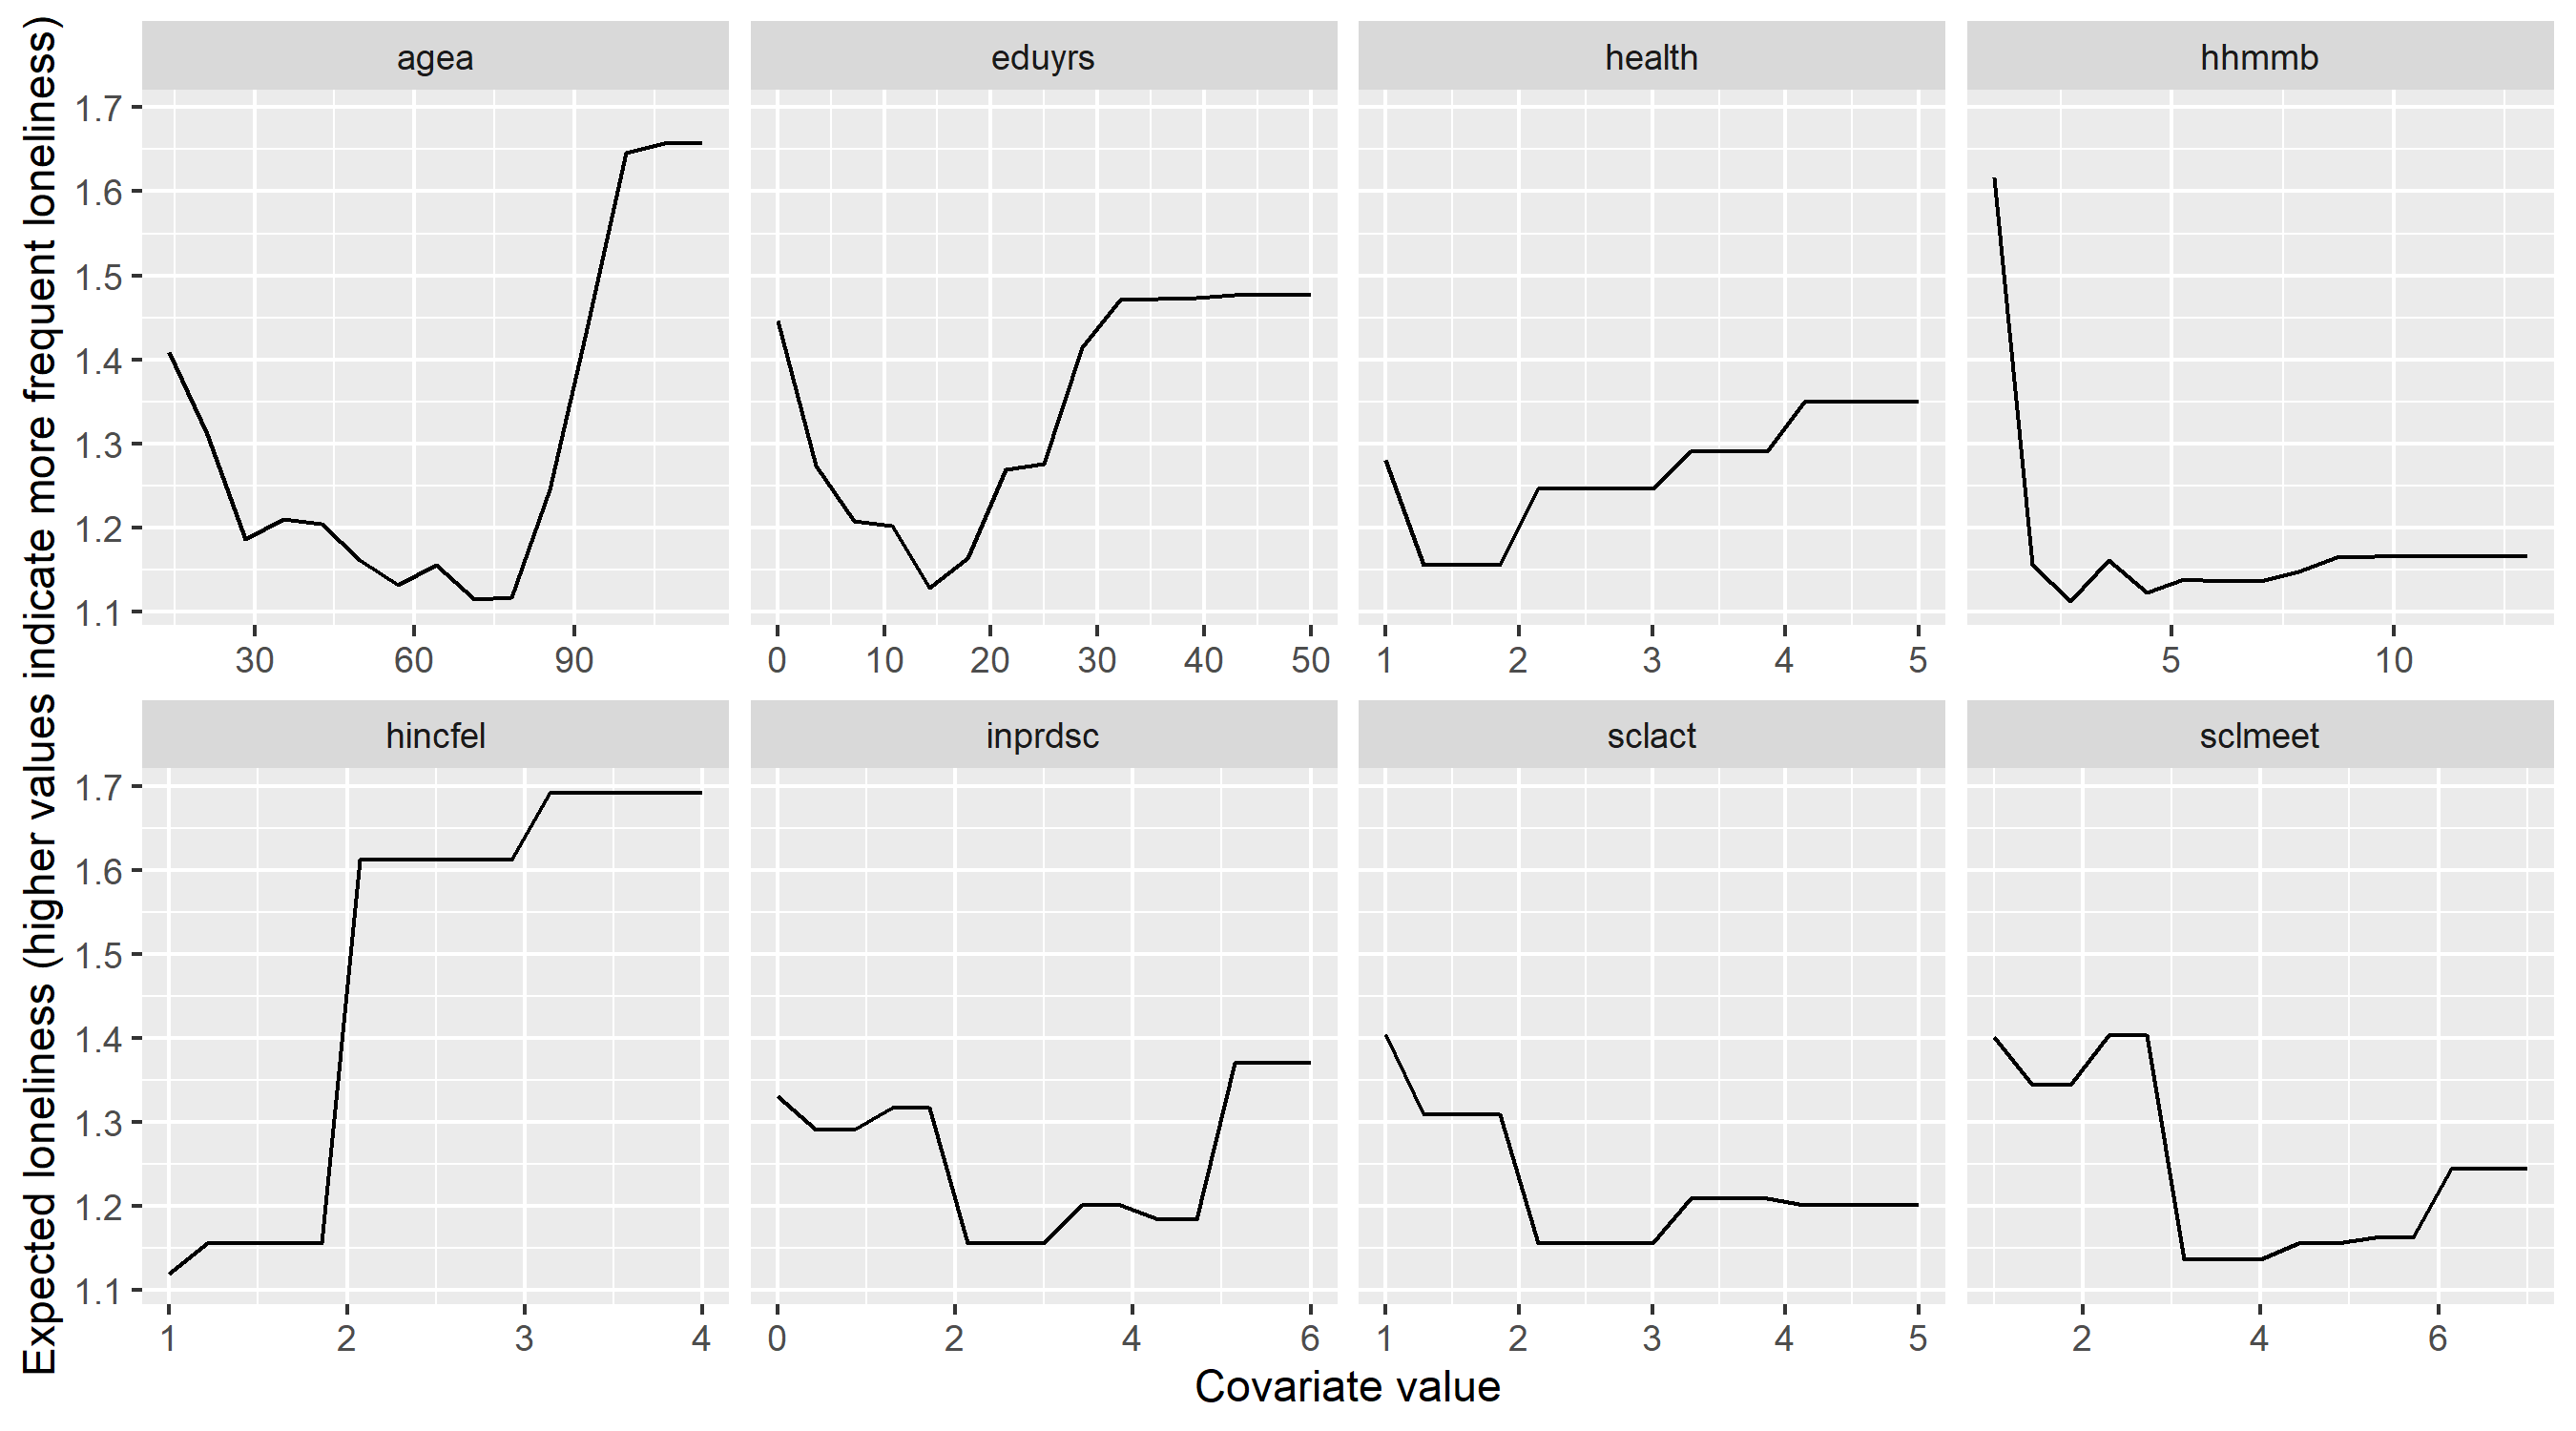
\includegraphics[width=0.8\textwidth]{fig_pdp_full.png}

  \raggedright
  \textit{Note.} Each panel shows the partial dependence of expected loneliness for one
  numerical predictor, computed with the remaining numerical predictors held at their
  medians and gender held fixed. The x-axis reports the covariate value and the y-axis
  reports the expected loneliness category; higher values indicate more frequent loneliness.
\end{figure}

\subsection{Incremental predictive value}

Table~\ref{tab:ipv} reports the five-fold test performance of the four nested ordinal
forests. Adding \code{inprdsc} or \code{sclact} individually produced small and inconsistent
changes in accuracy, $\kappa$, and MAE. Adding both together, however,
increased mean $\kappa$ from $.182$ to $.204$ ($\Delta = .022$), whereas changes in
accuracy and MAE were small. This non-additive
pattern suggests that intimate confidants (\code{inprdsc}) and broader social participation
(\code{sclact}) capture complementary dimensions of social connection whose joint predictive
value is visible primarily in ordinal agreement rather than in exact-category accuracy.

\begin{table}[H]
  \footnotesize
  \caption{Incremental Predictive Value of the Social-Connection Predictors}
  \label{tab:ipv}
  \begin{tabular}{lccc}
    \toprule
    Model & Accuracy & Weighted $\kappa$ & MAE \\
    \midrule
    Base & .716 (.009) & .182 (.009) & .360 (.017) \\
    Base + \code{inprdsc} & .719 (.007) & .187 (.014) & .356 (.017) \\
    Base + \code{sclact} & .717 (.008) & .175 (.015) & .359 (.017) \\
    Base + \code{inprdsc} + \code{sclact} & .717 (.008) & .204 (.017) & .357 (.017) \\
    \bottomrule
  \end{tabular}

  \vspace{6pt}

  \raggedright
  \textit{Note.} Values are means across five test folds (standard deviations in
  parentheses). Incremental change relative to the base model, with positive values
  indicating improvement (for MAE, a reduction in error): \code{inprdsc} = accuracy $+.002$,
  $\kappa$ $+.005$, MAE $+.004$; \code{sclact} = accuracy $+.001$, $\kappa$ $-.007$, MAE
  $+.001$; both = accuracy $+.000$, $\kappa$ $+.022$, MAE $+.002$. Increments were computed
  from unrounded means and may therefore differ slightly from differences between the rounded
  values shown.
\end{table}

\section{Discussion}

The present study examined whether confidant availability and peer-relative social
activity improve the prediction of concurrent loneliness beyond meeting frequency and
background characteristics. The model comparisons provided initial insight into the
underlying data structure: limited country-level variation indicated by the negligible
ICC suggests that most variation in loneliness occurred among individuals within
countries; the stronger performance of the ordinal forest compared to linear cumulative
link models could indicate meaningful nonlinearity embedded in the data. Importantly,
inclusion of both confidant availability and peer-relative social activity modestly
improved ordinal agreement, with smaller changes in accuracy and MAE. The full-sample
ordinal forest provided a complementary perspective by situating these social indicators
within respondents' wider life circumstances.

\subsection{Incremental predictive value}

The clearest improvement occurred when confidant availability and peer-relative social
activity were included together, whereas their separate contributions were small and
inconsistent. The joint gain suggests a possibility that the meaning of one social
indicator depends partly on the other resources a person has. Someone who participates
less than their peers but has trusted confidants may prefer a quieter social life,
whereas similar participation without anyone to confide in could reflect more extensive
disconnection. Considering both indicators may help distinguish these circumstances,
making more accurate predictions. Future research could further examine whether this
pattern involves identifying how resources compensate for one another, as well as when
they are jointly lacking.

A possible explanation for the smaller incremental contribution is that some
opportunities and constraints surrounding relationships may have already been captured
indirectly, as the baseline included background information from age and education to
living arrangements. The additional social indicators could therefore overlap with
information the model already possessed. For instance, having fewer confidants can be
closely associated with greater loneliness. Yet asking about confidants might add
relatively little if household size has already captured some related information about
everyday companionship or support.

\subsection{Social connections in everyday life}

The full-sample model is particularly relevant to understanding why these social
indicators add only modestly by placing them within the conditions of everyday life.
Although included as a background covariate, household size ranked the highest in the
feature-importance figure. It may capture important forms of connection that are woven
into everyday routines but easily overlooked, especially when social life is described
mainly through meetings and activities. Sharing a household can mean having someone
routinely available to exchange a few words, share a meal, or discuss an unexpected
difficulty, without arranging a separate social occasion. Moreover, at the fixed
covariate settings used, the household-size partial dependence profile showed a sharp
distinction between living alone and sharing a household, aligning with the
interpretation. Household size may also reflect partnership and family circumstances
that were not measured separately. Its importance invites a closer examination of what
shared living provides.

The prominence of age, income strain, and self-rated health similarly describes the
practical conditions needed. Relationships require ongoing resources and care as life
circumstances shift. However, financial and health constraints could limit people from
participating in social events, thus preventing new connections or making existing
connections harder to maintain. The plot for age further highlights the importance of
accounting for life stages. Higher predicted loneliness among younger respondents and
the oldest age groups is broadly consistent with earlier findings by Luhmann and Hawkley
(2016). Younger people may be establishing relationships and financial independence,
whereas older people may face changes in health or companionship.

Within those circumstances, confidant availability and peer-relative activity ranked
above meeting frequency. Related research has likewise highlighted confidant-based
support and satisfaction with contact alongside actual contact frequency (Amendola \&
von Wyl, 2025; Nicolaisen \& Thorsen, 2017). Though the present measures do not directly
establish relationship quality or satisfaction, their differing roles in the model
support examining social connection through more than one question. More specifically,
their partial dependence profile suggests that an important first step may be moving
beyond limited connection. The clearest differences occur between limited connection
and more established access to confidants or regular contact. Lower predictions as
activity approached that of peers are also consistent with the possibility that
perceived inclusion matters, although the measure does not directly assess belonging.

Interestingly, predicted loneliness did not continue to decline at the highest levels
of all three indicators. One possible interpretation is that additional social
connection matters most when it addresses an unmet relational need; once existing
relationships are sufficient, further increases may make less difference to loneliness.
Therefore, efforts to address loneliness could begin by identifying what people feel is
missing from their relationships. Another possibility concerns measurement. Having
several potential confidants does not establish that supportive conversations occurred
during the week assessed, and frequent participation need not feel satisfying. The
flattening or upturns may therefore reflect how little counts reveal about the
experience of relationships at higher levels. Nevertheless, further analyses are needed
to establish how stable these patterns are.

\subsection{Limitations and future directions}

Our incremental comparisons used a subsample of 10,500 respondents and one five-fold
partition due to computational constraints. Although 500 respondents per country
preserved country coverage, and identical respondents and folds supported comparable
evaluations, the estimates may depend on the particular sample and partition. Similarly,
importance was estimated from 1,000 training observations using one permutation per
predictor, leaving ranking stability uncertain. The partial dependence profiles were
evaluated at a single reference covariate configuration, and their shapes may differ
under other settings. These choices provided an exploratory description of the fitted
model. In the future, profiles averaged across respondents together with comparisons
across different covariate configurations would strengthen interpretation. Finally, the
cross-sectional design and single past-week item limit conclusions about temporal
direction and persistent loneliness. Longitudinal studies using repeated, multi-item
assessments could address these questions.

\section{Conclusion}

Based on ESS Round 7 data, confidant availability and peer-relative social activity
provided a modest joint improvement in loneliness prediction beyond meeting frequency
and background characteristics, mainly in ordinal agreement. The exploratory prominence
of household size, age, financial and health conditions also highlights the context in
which social connection occurs. Together, these findings suggest value in considering
how social resources fit together within people's lives and the conditions that make
them accessible. A useful next step is to measure unmet relational needs directly and
test whether they improve prediction beyond these broad indicators. This could help
distinguish needs for companionship, participation, or personal support. Ultimately, by
reducing mismatches between available support and people's relational needs, limited
resources for loneliness services could be used more effectively.

\newpage

\section{References}

\begingroup
\setlength{\leftskip}{0.5in}
\setlength{\parindent}{-0.5in}
\setlength{\parskip}{0pt}

Amendola, S., \& von Wyl, A. (2025). Trends in loneliness in 17 European countries
between 2006 and 2015: A secondary analysis of data from the European Social Survey.
\emph{Journal of Health Psychology}, \emph{30}(7), 1680--1697.
\url{https://doi.org/10.1177/13591053241278473}

Bergonzoli, G., Rossi, L., \& Masci, C. (2026). Ordinal mixed-effects random forests.
\emph{Journal of Classification}. \url{https://doi.org/10.1007/s00357-026-09558-1}

Christensen, R.~H.~B. (2022). \emph{ordinal---Regression models for ordinal data}
[Computer software]. R package version 2022.11-16.
\url{https://CRAN.R-project.org/package=ordinal}

Cohen, J. (1968). Weighted kappa: Nominal scale agreement provision for scaled disagreement
or partial credit. \emph{Psychological Bulletin}, \emph{70}(4), 213--220.
\url{https://doi.org/10.1037/h0026256}

ESS ERIC. (2014). \emph{European Social Survey Round 7 Data} [Data set]. Data file edition
2.3. NSD---Norwegian Centre for Research Data, Norway.
\url{https://doi.org/10.21338/ess7e02_3}

Grilli, L., \& Rampichini, C. (2011). Multilevel models for ordinal data. In \emph{Modern
analysis of customer surveys} (pp. 391--411). Wiley.
\url{https://doi.org/10.1002/9781119961154.ch19}

Hawkley, L.~C., \& Cacioppo, J.~T. (2010). Loneliness matters: A theoretical and
empirical review of consequences and mechanisms. \emph{Annals of Behavioral Medicine},
\emph{40}(2), 218--227. \url{https://doi.org/10.1007/s12160-010-9210-8}

Heu, L.~C., van Zomeren, M., \& Hansen, N. (2019). Lonely alone or lonely together? A
cultural-psychological examination of individualism--collectivism and loneliness in five
European countries. \emph{Personality and Social Psychology Bulletin}, \emph{45}(5),
780--793. \url{https://doi.org/10.1177/0146167218796793}

Hornung, R. (2020). Ordinal forests. \emph{Journal of Classification}, \emph{37}, 4--17.
\url{https://doi.org/10.1007/s00357-018-9302-x}

Luhmann, M., \& Hawkley, L.~C. (2016). Age differences in loneliness from late
adolescence to oldest old age. \emph{Developmental Psychology}, \emph{52}(6), 943--959.
\url{https://doi.org/10.1037/dev0000117}

McCullagh, P. (1980). Regression models for ordinal data. \emph{Journal of the Royal
Statistical Society: Series B (Methodological)}, \emph{42}(2), 109--127.
\url{https://doi.org/10.1111/j.2517-6161.1980.tb01109.x}

Nicolaisen, M., \& Thorsen, K. (2017). What are friends for? Friendships and loneliness
over the lifespan---from 18 to 79 years. \emph{The International Journal of Aging and
Human Development}, \emph{84}(2), 126--158.
\url{https://doi.org/10.1177/0091415016655166}

Perlman, D., \& Peplau, L.~A. (1981). Toward a social psychology of loneliness. In
S. Duck \& R. Gilmour (Eds.), \emph{Personal relationships: Vol. 3. Personal
relationships in disorder} (pp. 31--56). Academic Press.

R Core Team. (2025). \emph{R: A language and environment for statistical computing}.
R Foundation for Statistical Computing, Vienna, Austria.
\url{https://www.R-project.org/}

Tutz, G., \& Hennevogl, W. (1996). Random effects in ordinal regression models.
\emph{Computational Statistics \& Data Analysis}, \emph{22}(5), 537--557.
\url{https://doi.org/10.1016/0167-9473(96)00004-7}

Wright, M.~N., \& Ziegler, A. (2017). ranger: A fast implementation of random forests for
high dimensional data in C++ and R. \emph{Journal of Statistical Software}, \emph{77}(1),
1--17. \url{https://doi.org/10.18637/jss.v077.i01}

Yarkoni, T., \& Westfall, J. (2017). Choosing prediction over explanation in psychology:
Lessons from machine learning. \emph{Perspectives on Psychological Science}, \emph{12}(6),
1100--1122. \url{https://doi.org/10.1177/1745691617693393}

\endgroup

\end{document}
